\section{Traffic Shaping Tunnel}
\label{sec:design}

%\todo{Design goals look rather similar to Pacer.}
%The previous section describes an abstract differentially private traffic
%shaping strategy.
%We now present \sys's traffic-shaping tunnel.
%
A tunnel must address three requirements.
First, it must satisfy DP guarantees. For this, the tunnel~must complete DP
queries and prepare shaped packets within each interval, and it
must be able to transmit all payload bytes generated from an application within
a finite window length (as defined in the DP strategy).
%
Secondly, the payload and dummy bytes in the shaped packets must be
indistinguishable to an adversary. For this, the payload and dummy bytes must be
transmitted through a shared transport layer so that they are identically
acknowledged by the receiver and subject to congestion control and
loss recovery mechanisms.
%
Finally, the tunnel must provide similar levels of reliability,
congestion control, and loss recovery as expected by the application.

\if 0
A traffic shaping tunnel must address three requirements.
%{\bf R1.} It must ensure that the payload is unobservable to an adversary from
%the traffic shape. The packet sizes and timing may be correlated with
%application secrets or the application's sending or receiving rate (\ie flow
%control), which in turn may be secret-dependent.
{\bf R1.} Given a sequence of packets whose sizes and timing reveal the payload,
the tunnel must produce a packet sequence whose sizes and timing do not reveal
information about the payload.
{\bf R2.} It must protect against an adversary observing packets
along the entire path between the tunnel endpoints.
{\bf R3.} It must provide similar levels of reliability, congestion control, and
loss recovery as the original packet sequence.

R1 requires that the tunnel implements DP shaping correctly. Specifically,
it must complete DP decision making and preparation of a shaped buffer within
each interval (as defined in the DP shaping strategy). Moreover, it must be able
to transmit all payload bytes generated from an application within a finite
window length (defined in the DP shaping strategy).
R2 and R3 require that a tunnel implements padding in the outbound packets above
the transport layer so that it is delivered and acknowledged by the destination
and retransmitted upon loss in the same way as application payload.
%R2 requires that a tunnel must ensure that both payload and padding is delivered
%and elicit acknowledgements from the destination and, thus, must apply padding
%in the outbound packets before the transport layer packets are constructed.

One way to address all the requirements is to tunnel the transport layer
protocol between the application endpoints through {\sys}'s tunnel.
However, tunneling UDP through any protocol can be inefficient,
and tunneling
TCP through TCP can cause a TCP meltdown \cite{honda2005tcpovertcp,
tcp-meltdown}.
Tunneling TCP through UDP is insecure: TCP between the application end hosts
handles retransmission of lost payload bytes only,
not of any dummy bytes injected between the tunnel endpoints, making padding
observable.
\fi

%R1 requires that the tunnel must complete DP measurements and prepare shaped
%buffer within each decision interval, and it must be able to transmit all
%payload bytes generated from an application within a finite window length (as
%defined in the DP shaping strategy).
%R3 requires that the tunnel implements a transport protocol that subjects
%application's traffic to similar mechanisms as expected by the the application,
%and
%R2 requires that the dummy bytes are transmitted above the transport layer so
%that they are acknowledged by the destination and subject to the identical
%congestion control and loss recovery mechanisms as the payload bytes.

\Cref{fig:minesvpn-overview} shows the design of one endpoint of {\sys}’s
traffic shaping tunnel. A similar endpoint is deployed on the other end of
the tunnel.
%\ml{and bi-directional streams' privacy loss is the DP composition
%of the privacy loss in each direction}.
%The endpoints could be integrated with the end hosts or with a gateway at the
%edge of an organization’s network. Each tunnel is bidirectional, where the
%shape can be configured independently in each direction.
%
{The shape of the traffic in the tunnel can be configured independently
in each direction. The privacy loss in bidirectional streams is the DP
composition of the privacy loss in each direction.}

A tunnel endpoint consists of a shaping layer (Shaper) on top of QUIC, which
in turn runs on top of a standard UDP stack.
%\footnote{Instead of QUIC/UDP, {\sys} could also use a traditional TCP stack.}.
The tunnel endpoints establish a
bidirectional QUIC connection and generate DP-sized transmit buffers in fixed
intervals, which carry payload bytes from one or more application flows. In the
absence of application payload, a tunnel endpoint transmits dummy bytes, which
are discarded at the other endpoint. QUIC encrypts all outbound packets.
%Each tunnel is bidirectional, where the shape can be configured independently in
%each direction.

%An application interacts with the shaping layer through a set of per-flow queues
%carrying the application byte stream. Each flow is mapped to a pair of transmit
%and receive queues.

{\sys} adopts a transport-layer proxy architecture: each application
terminates a connection with its local tunnel endpoint. The application byte
stream is sent to the remote application over three piecewise connections: (i)
between the application and its local tunnel endpoint, (ii) between the
tunnel endpoints, and (iii) between the remote tunnel endpoint and the remote
application.
This ensures only one active congestion control and reliable delivery mechanism
in the tunnel and that all bytes are subject to identical mechanisms\footnote{
We discard tunneling TCP through TCP as it causes TCP
meltdown~\cite{honda2005tcpovertcp, tcp-meltdown}, or TCP through UDP as it is
unsafe.
(TCP between the application hosts would retransmit lost payload bytes
only, not any dummy bytes injected between the tunnel endpoints, making the
dummy bytes observable.)
%Tunneling TCP within TCP can cause a TCP meltdown \cite{honda2005tcpovertcp,
%tcp-meltdown}. Tunneling TCP through UDP is insecure: TCP between the
%application hosts would handle retransmission of lost payload bytes only, not of
%any dummy bytes injected between the tunnel endpoints, making the dummy bytes
%observable.
}.
%Moreover, payload and dummy bytes are subject to identical mechanisms in the
%tunnel, ensuring that they are indistinguishable to an adversary along the
%entire tunnel path.
%This architecture satisfies both the security and practical requirements of a
%traffic shaping tunnel.
%For ease of implementation, our prototype requires applications to explicitly
%connect to a tunnel endpoint.
%In principle, {\sys} can also transparently proxy application
%connections.

%An application interacts with the shaping layer through a socket connection. For
%each application connection, the shaping layer maintains a {\em buffering
%queue}, in which it accumulates the application's outbound byte stream before
%transforming it into a differentially-private packet sequence.

The application and the tunnel endpoint shown in \Cref{fig:minesvpn-overview}
could either be colocated on the same host or located on separate hosts.
%For example, the tunnel endpoint could be on a separate middlebox or integrated
%with a gateway at the edge of an organization's network.
In each case, the traffic between the application and the tunnel endpoint is
assumed to be unobservable to an adversary.
Our design (\S\ref{subsec:design-overview}) does not distinguish between the two
configurations.
Our implementation (\S\ref{sec:implementation}) assumes that the tunnel endpoint
is located on a separate middlebox. We discuss security in
\S\ref{subsec:impl-security} and alternate deployments in
\S\ref{subsec:design-discussion}.

\if 0
The tunnel endpoints could be integrated with the application hosts or with a
gateway at the edge of an organization’s network.
\todo{Although our implementation places tunnel endpoints on a middlebox, for
the purposes of our design, we do not distinguish between the locations of
application endpoints and tunnel endpoints; they could be located on the
same node, or they could be on different nodes as in our implementation.}
%Each tunnel is bidirectional, where the shape can be configured independently
%in each direction.
The security of the tunnel design relies on the key assumption that the traffic
between an application endpoint and the tunnel endpoint is unobservable to an
adversary.
%The security of the tunnel design relies on two key assumptions. First, the
%traffic between an application endpoint and the tunnel endpoint close to it is
%not observable to an adversary, as also mentioned in
%\S\ref{subsec:threat-model}. Secondly, the time required by the shaping layer to
%prepare the DP-sized buffers is independent of application secrets.
\fi

\subsection{Tunnel Design and Operations}
\label{subsec:design-overview}

\textbf{Tunnel setup and teardown.}
%When one endpoint of an application initiates communication with
%another endpoint, the initiator first establishes a {\sys} tunnel between the
%application endpoints before establishing communication with the receiver.
%Before establishing communication with a receiver, an initiator application
%first establishes a {\sys} tunnel between the application endpoints.
\update{Before applications can communicate with each other, a {\sys} tunnel
must be set up between their local tunnel endpoints.
The initiator application sends a configuration message to its local tunnel
endpoint with the source and destination IP addresses and ports, a reliability
flag, and a privacy descriptor.}
%\todo{and a tunnel lifetime}.
The reliability flag indicates if the tunnel should provide reliable delivery
semantics or not. The privacy descriptor indicates the DP parameters to be used
for shaping the tunnel traffic.
%\todo{The lifetime indicates the duration for which the tunnel transmits DP
%shaped traffic.}
%\mis{I don't understand the lifetime: this suggests that someone
%needs to know how long the tunnel needs to exist; doesn't it make more
%sense to have a timeout that says to shut down the tunnel after some
%period of inactivity?}
%\mis{About now I keep wanting to say, "No, it's the middlebox" ever time I
%see the word endpoint.  I think we need a sentence at the beginning of
%Section 4.1 (design overview) that says something like "Although our
%implementation places tunnel endpoints on a middlebox, for the purposes of our
%design, we do not distinguish between the locations of
%application endpoints and tunnel endpoints; they could be located on the
%same node, or they could be on different nodes as in our implementation.}

Upon receiving a configuration message, the Shaper establishes a QUIC
connection with the remote tunnel endpoint and configures the reliability
semantics and privacy parameters
%\todo{and tunnel lifetime}
for each direction.
It also initializes \todo{three types of bidirectional~streams in the tunnel:
control, dummy, and data streams}.
One {\em control stream} is used to transmit
messages related to the establishment and termination of a connection
between the application endpoints. A {\em dummy stream} transmits padding
in QUIC packets in the form of STREAM frames\footnote{We do not use QUIC's
PADDING frames as they do not elicit acknowledgements and hence are
distinguishable from STREAM frames \cite{rfc9000}.}.
%\ml{random pref: I would not make that a footnote.}
\todo{The tunnel pre-configures a finite number of data streams, which carry
payload bytes from one or more application flows.}

%\todo{After the expiry of the lifetime},
{When the tunnel is inactive for a period of time, one of the tunnel
endpoints initiates a termination sequence and closes all open QUIC streams and
the tunnel connection.}
%\ml{why? Doesn't that leak no user in the recent past? maybe it's ok?}


\textbf{Connection establishment and termination.}
Once a tunnel is ready, applications can establish and terminate connections
with each other, which is mediated by the tunnel.
When the initiator application runs a connection establishment handshake with
its local tunnel endpoint, the Shaper maps the application flow to
a per-flow buffering queue and one of the inactive QUIC data streams in the
tunnel, and notifies the remote tunnel endpoint.
The remote tunnel endpoint establishes a connection with the receiver
application and maps the receiver application's flow with the data stream.
The connection termination handshake is handled similarly by the tunnel
endpoints. The messages for connection establishment and termination are
transmitted over the control stream in the tunnel and shaped according to the
tunnel's parameters.
%Once a tunnel is ready, the initiator application runs a connection handshake,
%which is intercepted in the local tunnel endpoint.
%\todo{The Shaper maps the application flow to one of the inactive data streams
%in the tunnel.}
%%\todo{The Shaper establishes a new QUIC data stream in
%%the existing tunnel and maps the new application flow to the new stream.}
%The remote tunnel endpoint establishes a connection with the receiver and sets
%up the receiver's configurations in the QUIC tunnel.
%%\todo{When an application flow terminates, the tunnel closes the QUIC data
%%stream and the connections with the application endpoints.}
%\todo{When an application flow terminates, the tunnel unmaps the QUIC data
%stream and closes the connections with the applications.}
%\todo{The connection termination messages for applications}
%The stream setup and closing messages are shaped according to the tunnel's
%parameters. \am{Fix the red text.}
%\todo{If a tunnel is already exists between the source and destination IP
%addresses with the same configurations, the shaping layer maps the new
%application flow with one of the unused data streams in the existing tunnel.}
%{\todo{After the expiry of the lifetime}, one of the tunnel endpoints initiates
%a termination sequence and closes all open QUIC streams and the tunnel
%connection.}


\textbf{Outbound traffic shaping.}
%For each application flow, the Shaper maintains a {\em buffering
%queue}, in which it accumulates the application's outbound byte stream before
%transforming it into a differentially-private packet sequence.
The Shaper accumulates the outbound bytes of an application flow in a
buffering queue before it transmits them in packets whose sizes and timing
follow a distribution that guarantees DP.
Within a tunnel, the Shaper transmits bytes from all active flows into a
differentially-private packet sequence.
%The Shaper in a tunnel endpoint converts the byte stream of one or more
%application flows into a sequence of network packets whose sizes and timing
%follow a distribution that guarantees DP.
At periodic intervals, {called DP shaping intervals,} it performs a
DP query on the per-flow queues to determine the
number of bytes $\qlendp$ to be~transmitted according to the tunnel's DP
parameters. It prepares a {\em shaped buffer} consisting of $\payload$ payload
bytes and $\dummy$ dummy bytes, where $\payload$ is the minimum of $\qlendp$ and
the application bytes available in the buffering~queues, and $\dummy = \qlendp -
\payload$, which may lie between 0 and $\qlendp$. The Shaper then passes
the buffer with the position and length of the padding to QUIC.

QUIC transforms the shaped buffer into one or more STREAM frames based on the
congestion window, the flow window of the receiver endpoint, and the MTU
(maximum transmission unit). It
places the padding bytes into a dummy STREAM frame. QUIC packages the frames
into packets, whose length is at most MTU
minus the length of the headers and whose payload is
encrypted. QUIC forwards the packets to the UDP layer, which subsequently
transmits the prepared packets as quickly as it can, given the line rate of the
NIC.

To enforce \Cref{assumption:window}, the Shaper tracks the expiry time of
each byte enqueued in $\buffQ$ based on the arrival time and the neighboring
window length $\winlen$ configuration. The Shaper drops the untransmitted bytes
in the queue upon their expiry.

%\todo{{\sys} configures the {DP shaping} interval such that the Shaper can
%prepare each shaped buffer within the interval. If the preparation time for a
%buffer exceeds the interval, the Shaper discards the buffer. This ensures that
%the buffering queue length does not grow significantly, which in turn controls
%the overhead incurred due to DP shaping.}
%\am{Note this is secure only if delays due to cc. All other delays should be
    %properly masked.}
%

%%%%%%%%%%%%%%%%%%%%%%%%%%%%%%%%%
%% mentioned at the end of sec 3.
%%%%%%%%%%%%%%%%%%%%%%%%%%%%%%%%%
%We evaluate the impact of the buffering queue length and the DP
%shaping interval on privacy guarantees, bandwidth overheads, and latency
%overheads in \S\ref{sec:eval}.

\textbf{Inbound traffic processing.}
A tunnel endpoint receives shaped packets from the tunnel and applies inverse
processing on each packet.
QUIC receives the packet and
sends an ACK to the sender. Subsequently, it decrypts the packet, discards the
dummy frame, and forwards the payload bytes from the remaining STREAM frames to
the application.
%\as{Comment 7: we should add a paragraph here, explaining that the tunnel
%endpoint is modular. It does not necessarily require to be in a middlebox. We
%chose it to be in a middlebox for reasons we provide in next section.}

\subsection{Middlebox Implementation}
\label{sec:implementation}

\begin{figure}[t]
    \centering
    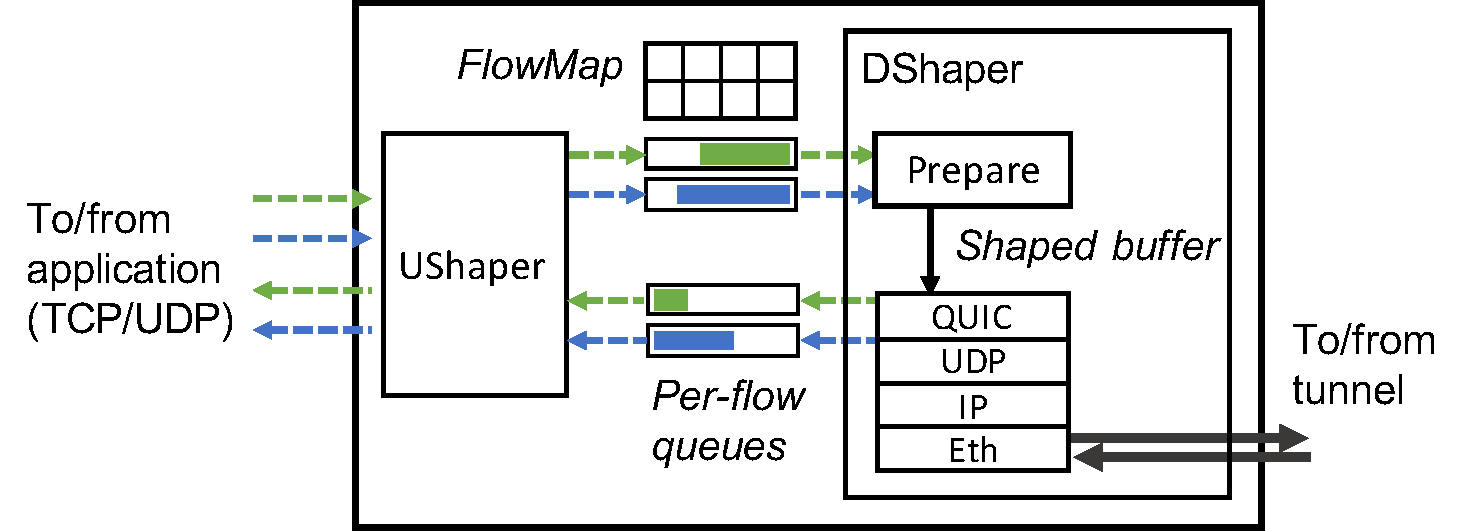
\includegraphics[width=\columnwidth]{middlebox-arch3.pdf}
    %    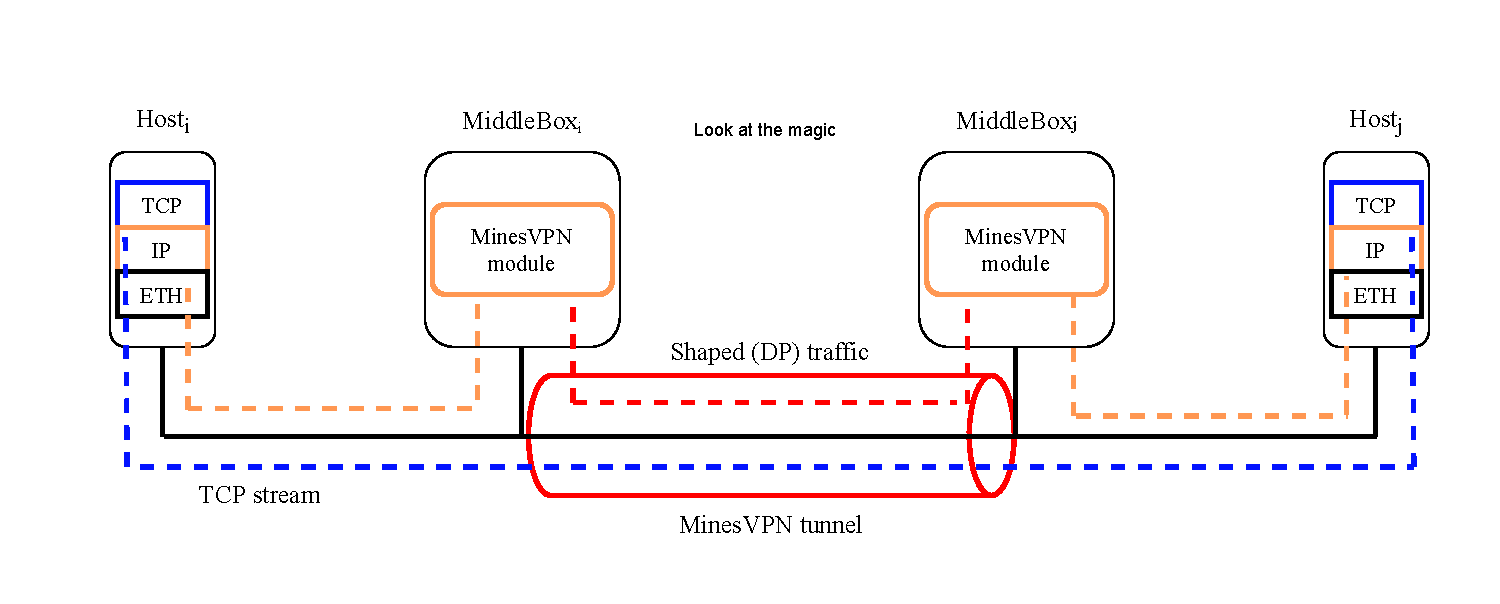
\includegraphics[width=\columnwidth]{figures/design.pdf}
    \caption{{\sys} middlebox design}
    \vspace{-0.4cm}
    \label{fig:minesvpn-impl}
\end{figure}

We present a middlebox-based {\sys} implementation.
%as shown in \Cref{fig:minesvpn-impl}.
%
%Recall from \S\ref{subsec:key-ideas}, a middlebox can support shaping for
%several applications and amortizes~the shaping cost among multiple flows that
%share the same tunnel.
%%Moreover, middleboxes can support ``long-term'' tunnels between
%%endpoints. Such tunnels may be set up, for instance, between organization
%%campuses to secure all communication between the campuses without the need for
%%modifying individual application hosts.
%
For ease of implementation, our prototype requires applications to explicitly
connect to the middleboxes.
In principle, {\sys} can transparently proxy application
connections.

%Following the proxy architecture, the middlebox splits the communication between
%two application endpoints over three transport connections:
%one between two middlebox endpoints that provides a tunnel and one between
%each application endpoint and its local middlebox.
In our implementation (see \Cref{fig:minesvpn-impl}), a middlebox consists of
two userspace processes. The
{\ushaper} mediates {\em unshaped} traffic between the applications and the
middleboxes. The {\dshaper} handles {\em DP shaped} traffic within the tunnel.

%\subsection{Components}
%\label{subsec:impl-mediation}
\textbf{UShaper.}
%The {\ushaper} mediates the unshaped traffic between one or more local
%application endpoints and the {\dshaper} using per-flow transmit and receive
%queues.
%It implements
The {\ushaper} implements a transport server (or client) for interfacing with
each local client (or server, respectively) application.
%\footnote{The {\ushaper} could also be a SOCKS5 proxy \cite{torpt}.}.
%\ml{random pref: wouldn't use a footnote here}
%The type of the transport endpoint depends on the application's choice of
%transport protocol.
For managing multiple flows, it shares a {\flowmap} table with the {\dshaper},
which consists of an entry for each end-to-end flow. Each entry maps the
piecewise connections with
%the associated sockets of {\ushaper} and {\dshaper}, a
a pair of transmit and receive queues to carry the local application's byte
stream, and shaping configurations (\eg privacy descriptor) provided by an
%\todo{(\eg privacy descriptor, tunnel lifetime)} provided by an
application at the time of flow registration.
%The transmit queues of the end-to-end flows mapped to a single tunnel connection
%correspond to the tunnel's buffering queue, on which tunnel's DP guarantees
%rely.

The {\ushaper} receives the outbound traffic from a sender application
and enqueues the byte stream into a per-flow transmit queue shared with the
{\dshaper}.
It also dequeues bytes from a per-flow receive queue, repackages them
into transport packets and sends them to the receiver application.

%\if 0
\begin{figure}[t]
    \centering
    %    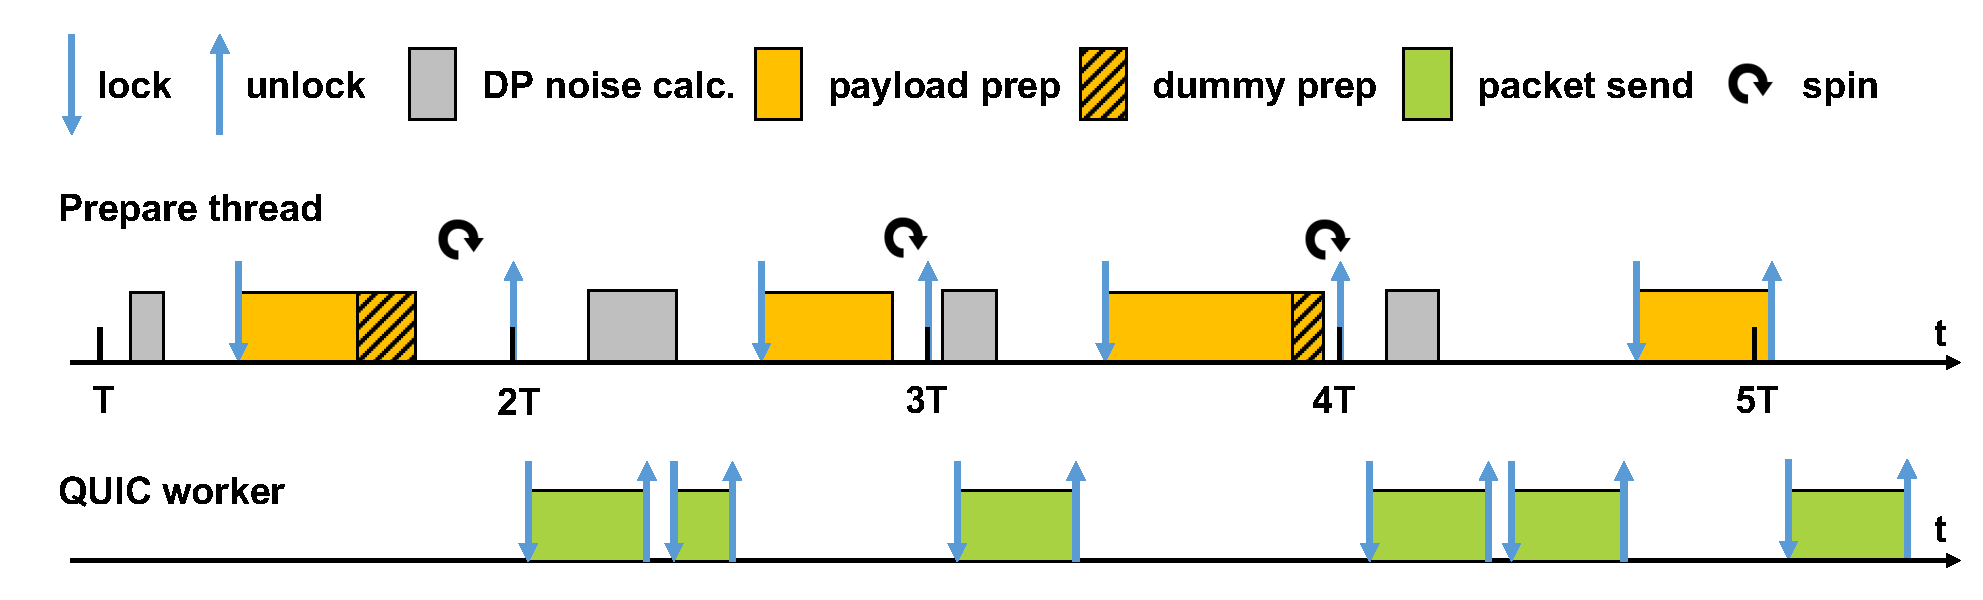
\includegraphics[width=\columnwidth]{figures/schedule.pdf}
    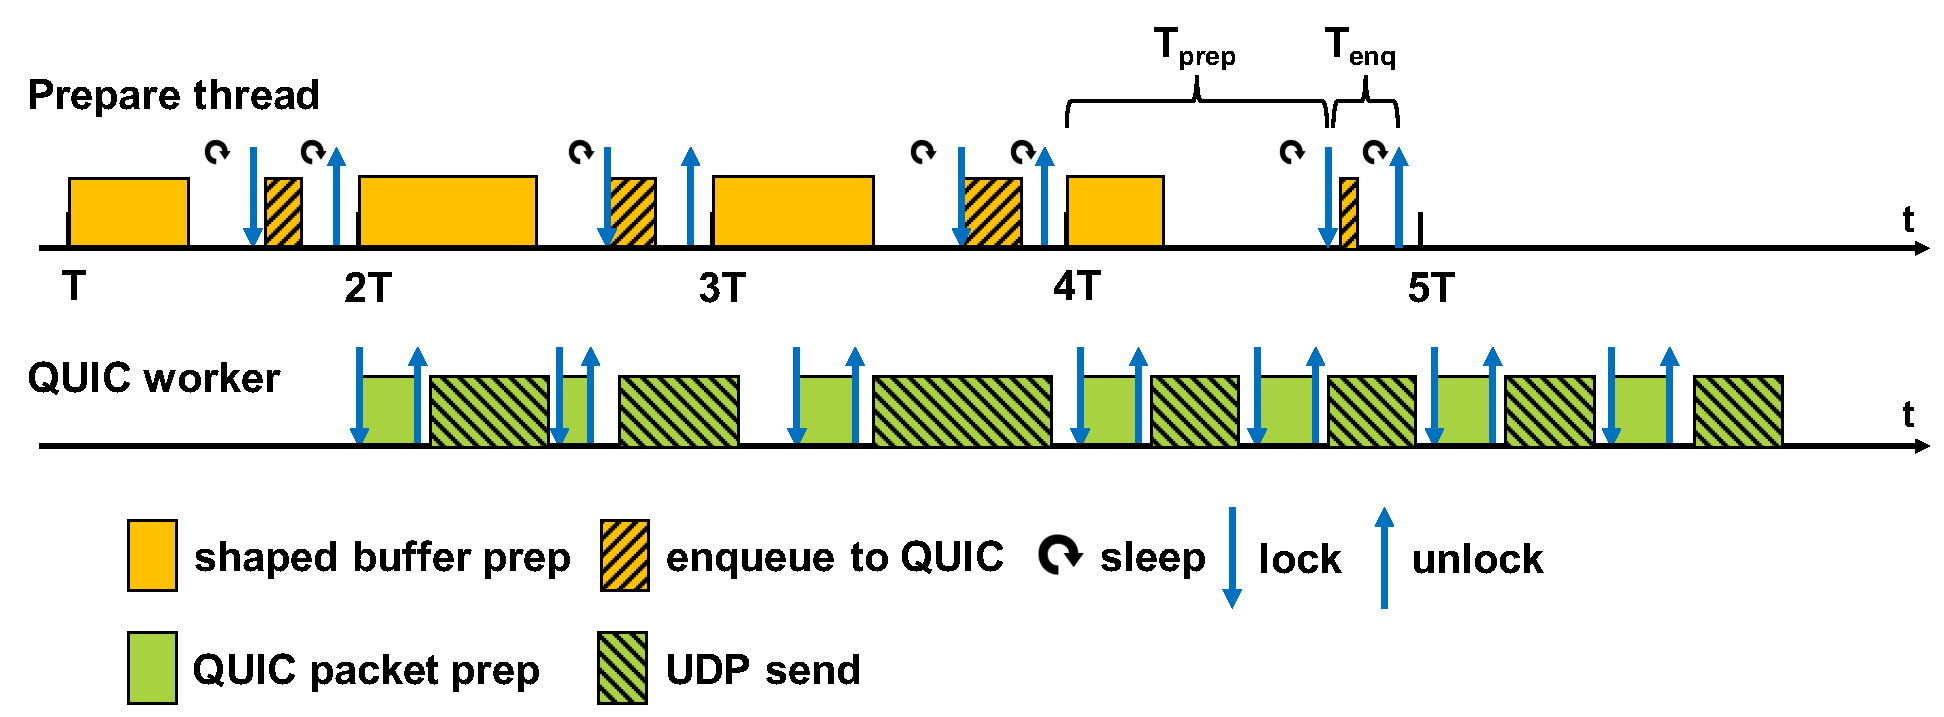
\includegraphics[width=\columnwidth]{schedule5.pdf}
    \caption{{\dshaper} schedule}
    \vspace{-0.4cm}
    \label{fig:middlebox-schedule}
\end{figure}
%\fi

\textbf{DShaper.}
%
The {\dshaper} consists of a {\prepare} thread and a QUIC
worker thread.
The {\prepare} thread instantiates a QUIC client/server to establish
a tunnel with the remote middlebox and implements the DP shaping logic.
%On~the transmit side, {\prepare} examines the number of bytes in each
%per-flow transmit queue, determines the number of bytes to transmit,
On the transmit side, {\prepare} {prepares shaped buffers based on DP
queries on the transmit queues}
and then submits shaped buffers to the QUIC worker for transmission.
On the receive size, the QUIC worker transmits ACK frames to the sender
and then decrypts the QUIC packets, extracts the STREAM frames, and copies
bytes (including dummy bytes) from each frame into the appropriate per-flow
receive queue.

%\noindent
\textbf{Ensuring secret-independent shaping.}
%\as{Comment 1.1: We should rewrite this section from scratch, showing that all
%we perform is a best-effort guarantee.}
%\label{subsec:impl-shaping-security}
%\Cref{fig:middlebox-schedule} illustrates the schedule of operations on
%{\prepare}
%and QUIC worker threads on the outbound path.
%The green and orange boxes represent data-independent and data-dependent
%operations, respectively.
%\todo{
%To enforce DP guarantees, intuitively, the middlebox must ensure that {\em
%an adversary observes $\qlendp$ bytes in each transmit interval $\dpintvl$.}
To enforce DP guarantees, {\dshaper} should {\em transmit} exactly $\qlendp$
bytes in each DP shaping interval $\dpintvl$.
%\ml{not really right? It's that it observes a number of bytes---and any
%observable quantity---that is a post-processing of the DP measurements. Hence,
%any observable quantity cannot depend on application data other than throught
%the DP measurements.}
%}
%
\if 0
Let us first understand the factors that might prevent the middlebox from
guaranteeing this property.
Even though an application is physically isolated from the middlebox and can
encrypt its data (\eg using end-to-end TLS), its flow control behavior could be
secret-dependent and could affect the middlebox's execution.
For instance, the presence or absence of payload traffic from an application
can affect the time {\dshaper} requires to prepare the shaped buffers.
\fi
%
%Ensuring the high-level goal mentioned above requires that
This would require ensuring:
{\bf P1.} {\prepare} computes $\qlendp$, allocates and prepares a buffer
of length
$\qlendp$, and passes the buffer to the QUIC worker within $\dpintvl$,
{\bf P2.} the QUIC worker prepares encrypted packets from the buffer and sends
them to UDP, such that the total payload size of the QUIC packets prepared in
$\dpintvl$ is $\qlendp$, and
{\bf P3.} the~UDP stack transmits packets totaling to $\qlendp$ payload bytes
to the NIC in $\dpintvl$.
Enforcing all these properties would require a constant-time implementation for
each step, which is non-trivial, or a strict time-triggered schedule
for each step, which would significantly reduce link utilization and increase
packet latencies.
%transmission latencies.
%Moreover, the value of $\dpintvl$ required would be large to account for
%potential secret-dependent (\eg flow control) as well as secret-independent
%delays (\eg congestion control).
%This would significantly increase packet transmission latencies.

%\todo{Thanks to DP post processing, however, it suffices to ensure that the
%middlebox {\em prepares} a shaped buffer based on a DP measurement $\qlendp$
%within each time interval $\dpintvl$, \ie property P1. As long as the shaped
%buffers are transformed into network packets independently of the DP
%measurement, the sizes and timing of network packets need not be constrained in
%any way.
%}
\todo{Thanks to DP post processing, however, it suffices to ensure the property
P1,
%\ie that {\dshaper} {\em prepares} a shaped buffer based on a DP measurement
%$\qlendp$ within each time interval $\dpintvl$,
and {\bf P4.} that the QUIC worker transforms the shaped buffer into network
packets independently of the
%\ml{\sout{DP measurement in {\dshaper}}
application data.
%}.
%\ml{\sout{With this, the sizes and timing of network packets need not be
%constrained in any way.}
No other constraint on the sizes and timing of network packets is required to preserve DP.
%}
}

Satisfying P1 involves one challenge. Although the application is physically
isolated from the middlebox, its flow control behavior could be
secret-dependent and could affect the middlebox's execution.
For instance, the presence or absence of payload traffic from an application
can affect the time {\dshaper} requires to prepare the shaped buffers.

%{\dshaper} instead provides the following guarantees. \ml{this makes it sounds
%like we provide weaker than ideally needed guarantees. But we don't! We provide
%what we need to make the observable quantities be a data independent
%post-processing of DP measurements. If the above framing I suggested sounds
%good, this statement probably needs to not be an instead.}
Thus, {\dshaper} satisfies P1 as follows (see \Cref{fig:middlebox-schedule} for
reference).
%The {\dshaper} provides two guarantees.
First, {\prepare} {guarantees that $\qlendp$ is computed with a DP query
in each interval}.
Secondly, {\prepare} guarantees that a shaped buffer of length $\qlendp$ is {\em
prepared} within a fixed time $\dpintvl_{prep}$ within each interval.
Thirdly, {\prepare} locks the shaped buffer for a fixed time,
$\dpintvl_{enq}$, during which it enqueues the buffer for a QUIC
worker.
This ensures that~the buffer is completely enqueued before QUIC starts
transmitting it and that QUIC receives the buffer only at fixed delays.

%\todo{
We empirically profile the time taken by {\prepare} for preparing and enqueueing
shaped buffers for various DP lengths. We set $\dpintvl_{prep}$ and
$\dpintvl_{enq}$ to maximum values determined from profiling, and $\dpintvl$ to
the sum of these maximum values, \ie $\dpintvl_{max}$.
If {\prepare} takes time less than
$\dpintvl_{prep}$ (or $\dpintvl_{enq}$, respectively) to prepare (or enqueue) a
shaped buffer, it sleeps until the end of the interval before moving to the next
phase.
%}
%\todo{We empirically profile the maximal time $\dpintvl^{max}_{prep}$ and
%$\dpintvl^{max}_{enq}$ taken by {\prepare} for preparing and enqueueing shaped
%buffers for various DP sizes. We set $\dpintvl_{prep} = \dpintvl^{max}_{prep}$,
%$\dpintvl_{enq} = \dpintvl^{max}_{enq}$, and $\dpintvl = \dpintvl^{max}_{prep} +
%\dpintvl^{max}_{enq}$. If {\prepare} takes time less than
%$\dpintvl^{max}_{prep}$ (or $\dpintvl^{max}_{enq}$, respectively),
%to prepare (or enqueue) a shaped buffer,
%it sleeps until the end of the interval before moving to the next
%phase.}
%\am{Too symbol heavy?}


%{\dshaper} instead provides two guarantees.
%%The {\dshaper} provides two guarantees.
%First, {\prepare} guarantees that each shaped buffer is {\em prepared} within a
%fixed time interval $\dpintvl$.
%\todo{For this, we empirically profile the maximal time taken $\dpintvl_{max}$
%by {\prepare} until
%buffer preparation for various DP sizes and set $\dpintvl$ to this
%$\dpintvl_{max}$. If {\prepare} takes lesser time than $\dpintvl_{max}$ to
%prepare a transmit buffer, it sleeps until the end of the interval, at which
%point it starts enqueueing the buffer to QUIC.}
%Secondly, QUIC's packetization remains data-independent. For this, {\prepare}
%synchronizes with the QUIC worker on the the transmit buffers,
%%the preparation of buffers to be transmitted,
%ensuring that QUIC cannot receive fewer bytes than the computed DP
%size of the interval before it sends packets to the network. F
To satisfy P4,
%Additionally,
{\prepare} and QUIC worker threads run on separate cores
sharing only the shaped buffers.
%{\ushaper} runs on yet a different core, shares only the
%{\flowmap} and the per-flow queues with {\dshaper}.
{\ushaper} runs on yet a different core and shares the {\flowmap} and the
per-flow transmit queues containing unshaped traffic only with {\prepare}. It
shares the per-flow receive queues with the QUIC worker, but they contain only
shaped frames from the QUIC worker.
\update{Finally, we assume that QUIC encrypts and decrypts shaped
buffers in constant-time.}
With this, the execution of the QUIC worker becomes independent from {\prepare}
and secret-independent overall.
%
%In summary, variations in {\prepare}'s execution due to the state of the
%per-flow queues are masked by $\dpintvl_{max}$,
%%\as{comment 1.1: this maximum value is not necessarily guaranteed wrost-case
%%and might be violated in execution.}
%while QUIC's execution depends only on shaped buffers \update{and constant-time
%crypto}, and thus is secret-independent.
Consequently, the QUIC worker and the UDP stack can packetize the shaped buffers
and transmit the packets at link speed, and any variance in packet
transmit times constitute post-processing noise.
%Consequently, the packetization of shaped buffers in the QUIC worker and the UDP
%stack is secret-independent and any variations in packet transmit times
%%induced due to their execution
%constitute post-processing noise.

\textbf{Limitations.}
Our prototype has two limitations in enforcing secret-independent timing.
First, our QUIC implementation uses
standard OpenSSL, which may not provide constant-time crypto. However, QUIC can
be modified to adopt a constant-time crypto library~\cite{hacl,libsecp256k1} to
overcome this limitation.
Secondly, it is difficult to find the true maximum values of
$\dpintvl_{prep}$ and $\dpintvl_{enq}$ on general-purpose desktops. If
{\prepare}'s execution exceeds the profiled max values, it violates the
theoretical DP guarantees. However, we note that it is difficult to practically
exploit these violations for inferring traffic secrets.

\if 0
A remaining concern could be leaks via internal side channels in the middlebox
that cause {\dshaper} to fail to prepare the expected amount of data within a
scheduled interval.
For instance, {\dshaper}'s execution could be influenced by microarchitectural
state (\eg caches, memory and PCI buses, write buffers, interrupts) based on the
application's flow control.

We have not been able to exploit such side channels to identify traffic content.
Nevertheless, such side channels could be eliminated via resource partitioning,
performance isolation, and constant-time implementation techniques
\cite{liu2016catalyst, coppens2009practical, zhang2011predinteractive,
    almeida2016verifying}.
\fi

\if 0
A remaining concern could be leaks via internal side channels in the middlebox
that cause {\sys} to fail to transmit the expected amount of data within a
scheduled interval. Even though an application is physically isolated from the
middlebox and may encrypt its data (\eg using TLS for the end-to-end
connection), the application’s flow control could be secret-dependent and could
affect {\sys}'s execution.

\todo{For instance, flow control affects the number of payload bytes available
for transmission and, consequently, the amount of padding that may be added to a
segment. Processing payload and dummy bytes could take different amounts of
time.} Secondly, the execution of the Shaper could be influenced by interrupts
or microarchitectural state (\eg caches, memory and PCI buses, internal write
buffers) based on the presence or absence of payload traffic from the
application.
\fi

\if 0
\subsection{Scheduling Across Tunnels}
{When transmitting traffic on multiple tunnels, {\sys} must ensure that the
unshaped traffic of one tunnel is not leaked to another tunnel. For this, {\sys}
must isolate the tunnels from each other in the middlebox.
%Based on \S\ref{subsec:impl-shaping-security}, we require that the {\prepare}
%and QUIC worker threads must be performance isolated from {\ushaper} in each
%tunnel, (ii) the timing of {\prepare} must be masked to secret-independent
%times.
Thus, {\sys} partitions the middlebox cores into three groups, each core group
hosting the {\ushaper} process, the {\prepare} threads, and the QUIC worker
threads from different tunnels.
Furthermore, {\sys} uses a TDMA schedule among the {\prepare} threads, while
{padding} each thread's execution to a secret-independent time.
%In {\sys}, only the {\dshaper} components need to be isolated. {\sys} uses a
%TDMA to schedule the {\dshaper} processes of different tunnels.
Since each {\prepare} thread enqueues shaped buffers at secret-independent
times, the QUIC workers can subsequently package the buffers into packets and
transmit the packets across multiple tunnels following any arbitrary schedule.}
%
{Determining optimal TDMA schedules and their adaptation to the changing
number of active tunnels is left to future work.}
\am{Not implemented, remove?}
\fi
